% This file should only be \input{} in a document that loads the tikz package
% Do not compile this file directly with pdflatex

\begin{figure}
    \centering
    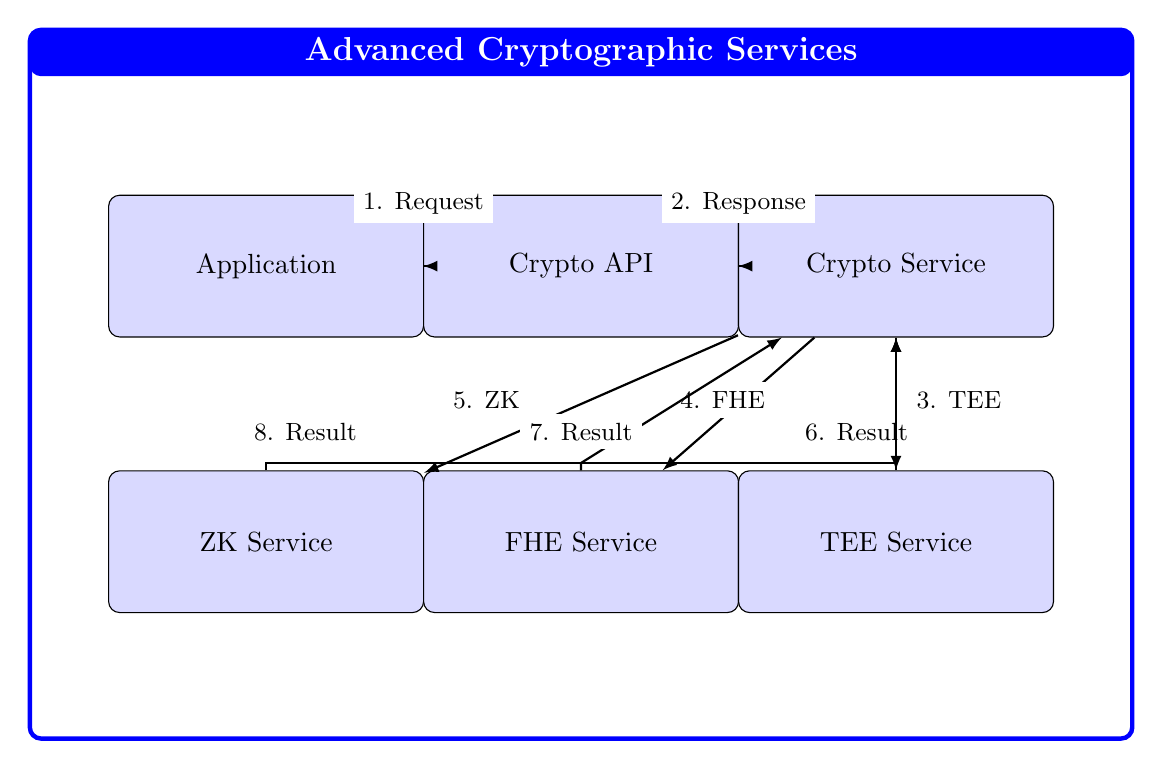
\begin{tikzpicture}[
        % Simple clean styling
        box/.style={draw, fill=blue!15, rounded corners, minimum width=4cm, minimum height=1.8cm, align=center},
        % Clean label style
        label/.style={font=\small, fill=white, draw=none, align=center},
        % Clean arrow style
        arrow/.style={->, >=latex, thick}
    ]
    
    % Define the main container
    \node[draw=blue, rounded corners, minimum width=14cm, minimum height=9cm, ultra thick] (container) {};
    
    % Add title
    \node[fill=blue, text=white, font=\large\bfseries, minimum width=14cm, rounded corners, anchor=north] at (container.north) {Advanced Cryptographic Services};
    
    % SIMPLIFIED LAYOUT - Grid arrangement
    % Top row - main components
    \node[box] (app) at (-4, 1.5) {Application};
    \node[box] (api) at (0, 1.5) {Crypto API};
    \node[box] (service) at (4, 1.5) {Crypto Service};
    
    % Bottom row - service components
    \node[box] (zk) at (-4, -2) {ZK Service};
    \node[box] (fhe) at (0, -2) {FHE Service};
    \node[box] (tee) at (4, -2) {TEE Service};
    
    % SIMPLIFIED CONNECTIONS WITH CLEAR LABELS
    
    % App to API
    \draw[arrow] (app) -- (api);
    \node[label] at (-2, 2.3) {1. Request};
    
    % API to Service
    \draw[arrow] (api) -- (service);
    \node[label] at (2, 2.3) {2. Response};
    
    % Service to specialized services
    \draw[arrow] (service) -- (tee);
    \node[label] at (4.8, -0.2) {3. TEE};
    
    \draw[arrow] (service) -- (fhe);
    \node[label] at (1.8, -0.2) {4. FHE};
    
    \draw[arrow] (service) -- (zk);
    \node[label] at (-1.2, -0.2) {5. ZK};
    
    % Return paths
    \coordinate (tee_return) at (3.5, 0);
    \draw[arrow] (tee) -- ++(0, 1) -| (service);
    \node[label] at (3.5, -0.6) {6. Result};
    
    \coordinate (fhe_return) at (0, 0);
    \draw[arrow] (fhe) -- ++(0, 1) -- (service);
    \node[label] at (0, -0.6) {7. Result};
    
    \coordinate (zk_return) at (-3.5, 0);
    \draw[arrow] (zk) -- ++(0, 1) -| (service);
    \node[label] at (-3.5, -0.6) {8. Result};

    \end{tikzpicture}
    \caption{Advanced Cryptographic Services Architecture}
    \label{fig:crypto-services}
\end{figure} 